\documentclass{rapportCS}
\usepackage{lipsum}
\usepackage{amsmath}
\usepackage{amsfonts}
\usepackage{amssymb}
\usepackage{enumitem}
\usepackage{comment}
\usepackage{tikz}
\usetikzlibrary{positioning, arrows.meta, decorations.pathreplacing}
\setlength{\marginparwidth}{2cm}
\usepackage{todonotes}
\setlist[itemize]{topsep=0pt, itemsep=0pt}

\title{End-of-Studies Internship Report Martini}

\begin{document}
  
% Informations du rapport 

\logoentreprise{logos/logoICM.png} %Logo de l'entreprise

\titre{Developing simulation and statistical evaluation tools for a non-linear mixed-effect model}

\mention{CentraleSupélec - Mention Sciences des données et de l'information \& Filière Métiers de la Recherche}
\master{Master MVA} % Nom du master
 

\eleve{Jean-Vincent Martini}  
 
\dates{April -- September 2026}   
 
% Informations tuteurs écoles
\tuteurecole{
    SDI: \textsc{Arthur Tenenhaus} \\
    arthur.tenenhaus@centralesupelec.fr \\
    FMR: \textsc{Vincent Mousseau} \\ 
    vincent.mousseau@centralesupelec.fr \\
    MVA: \textsc{Raphaël Porcher} \\
    raphael.porcher@aphp.fr
} 

\tuteurentreprise{
    \textsc{Sophie Tezenas du Montcel} \\
    sophie.tezenas@aphp.fr 
}

% Initialisation 
        
\fairemarges %Afficher les marges
\fairepagedegarde %Créer la page de garde
\setcounter{figure}{0}

\todo{ATTENTION AUX PARTIES CS ONLY: RECUL ETHIQUE, GRILLE DE COMPETENCES, etc. POSSIBLEMENT A RAJOUTER ENSUITE.}

% Abstract 
\begin{abstract}
This internship was carried out within the ARAMIS team at the Paris Brain Institute (ICM) and focused on the development of simulation and statistical evaluation tools for Leaspy, an open-source Python library dedicated to the analysis of multivariate longitudinal data in neurodegenerative diseases. Leaspy relies on non-linear mixed-effects models to reconstruct disease progression trajectories, align patients on a common latent disease timeline, and estimate individual progression parameters from repeated clinical observations.

The main objective of this work was to extend the simulation capabilities of Leaspy to its joint model, which simultaneously models longitudinal outcomes and time-to-event data through a shared latent disease age. While simulation tools already existed for the standard logistic model, no integrated implementation was available for the joint model. The internship therefore involved designing and implementing a simulation pipeline compatible with this framework, including event-time generation, management of censoring, support for competing events, and integration with the library's existing \texttt{estimate} and \texttt{simulate} interfaces.

A second major contribution consisted in developing a validation framework based on repeated simulation and re-estimation, in order to assess the self-consistency of the implementation and the statistical recovery of both population and individual parameters. This evaluation made it possible to identify which parameters are robustly recovered and which remain difficult to estimate in moderate-sample regimes, especially in the survival and latent-source components of the model.
\end{abstract}
\newpage 

\section*{Acknowledgements}   

I would like to thank Sophie Tezenas du Montcel, team leader and scientific director of this internship, for welcoming me into her research group and for her guidance throughout the project.

I also thank my supervisors Maylis Tran and Sofia Kaisaridi for their availability, their constructive feedback during our weekly meetings, and their support on both the scientific and software development aspects of the work.

I also wish to thank the members of the {ARAMIS team} for the stimulating and interdisciplinary working environment they foster. The exchanges I had with researchers, engineers, and fellow interns enriched both my understanding of computational neuroscience and my daily experience at the institute.

On the academic side, I would like to thank my school tutors, {Arthur Tenenhaus} (SDI) and {Vincent Mousseau} (FMR), for their follow-up and advice throughout the internship.

Finally, I extend my thanks to the {Paris Brain Institute (ICM)} and {INRIA} for providing the institutional and computational resources that made this work possible, as well as to the open-source contributors of the {Leaspy} library, whose prior work laid the foundations for my own contributions.
\newpage

% Table des matières 

\tableofcontents
\newpage   

% Introduction 

\section{Introduction} 

This end-of-studies internship was carried out from April to September 2026 at the Paris Brain Institute (ICM), located at the Pitié-Salpêtrière Hospital in Paris. The ICM is an internationally recognized research center dedicated to the understanding and treatment of neurological and psychiatric diseases. Its structure brings together clinicians, biologists, statisticians, computer scientists and engineers within a highly interdisciplinary environment, with the objective of fostering close interactions between methodological innovation and clinical applications.

The internship took place within the ARAMIS team (Algorithms, Models and Methods for Images and Signals), a joint team between the ICM and INRIA. ARAMIS develops computational and statistical tools for the analysis of brain data, with a particular focus on modeling disease progression in neurological disorders such as Alzheimer's disease, Parkinson's disease, Huntington's disease or amyotrophic lateral sclerosis. More specifically, I joined the longitudinal modeling group, whose research focuses on non-linear mixed-effects models for multivariate longitudinal data. This group combines expertise in statistics, machine learning and neuroscience to design models capable of capturing the temporal dynamics and inter-individual heterogeneity that characterize disease progression.

In this context, the internship was centered on Leaspy (LEArning Spatiotemporal Patterns in Python), an open-source Python library developed by ARAMIS and its collaborators for the statistical analysis of longitudinal clinical data. Leaspy aims at reconstructing disease trajectories from repeated patient measurements, aligning individuals onto a common disease timeline, and producing clinically interpretable quantities such as subject-specific disease stage or progression speed. The library already provides a mature implementation of several models and algorithms for fitting, personalization, trajectory estimation and, in some cases, simulation. However, as the methodological scope of Leaspy has expanded, especially with the recent development of a joint model linking longitudinal outcomes and survival data, the need for robust software tools for simulation and statistical evaluation has become increasingly important.

Indeed, simulation plays a central role in the development of complex statistical models. Unlike real clinical datasets, simulated datasets provide access to the ground truth: the true parameter values and latent variables are known by construction. They therefore make it possible to assess whether an estimation procedure is unbiased, whether individual parameters are accurately recovered, and whether an implementation behaves as expected under controlled conditions. In the specific case of Leaspy, this need is even stronger because the models are non-linear, involve latent random effects, and rely on computationally intensive estimation procedures such as MCMC-SAEM. Extending simulation capabilities to the joint model and designing tools to evaluate its statistical behaviour are thus both methodological and practical priorities.

The main objective of this internship was therefore to contribute to the development of simulation and statistical evaluation tools for Leaspy, with a particular focus on the joint model. Concretely, the work consisted in extending the simulation pipeline to settings involving longitudinal data jointly modeled with time-to-event outcomes, integrating these developments into the existing software architecture, and validating them through dedicated numerical experiments. Beyond the implementation effort itself, the internship also aimed at assessing the self-consistency of the model and estimation procedures through simulation-based validation studies.

More broadly, this work lies at the intersection of statistical modeling, scientific computing and software engineering. Because Leaspy is an open-source research library intended to be used both by methodologists and by applied researchers, contributing to it requires not only implementing new methodological features, but also ensuring code reliability, reproducibility, usability and documentation quality. In that respect, the internship included several additional contributions that are not detailed in the core chapters of this report: reviewing pull requests submitted to the library, writing and improving unit and functional tests, improving parts of the documentation, and preparing and leading a workshop on longitudinal data with a particular emphasis on simulation within Leaspy. These activities were an important part of the internship, as they contributed to the overall robustness, maintainability and dissemination of the software.

This report focuses primarily on the methodological and technical contributions related to simulation and evaluation for the joint model. It first presents the scientific and software context of the Leaspy library, as well as the motivations for simulation studies in this framework. It then introduces the joint model in more detail, describes the simulation algorithm implemented during the internship and the adaptations made within Leaspy, and finally reports a validation study designed to assess parameter recovery and the consistency of the overall pipeline. Through these developments, the internship aimed to strengthen both the methodological foundations and the practical usability of Leaspy for future research on longitudinal disease progression modeling.
\newpage 

% Sections 

\section{Context on the Leaspy library}

Neurodegenerative diseases are characterized by a slow and complex evolution, involving dozens to hundreds of heterogeneous clinical and biological markers such as continuous scores, discrete or ordinal assessments, censored survival outcomes, and high-dimensional modalities such as structural MRI or PET imaging, that evolve jointly over time. This complexity is further compounded by substantial inter-individual heterogeneity: patients sharing the same diagnosis can exhibit markedly different symptom profiles, progression rates, and responses to treatment. Modeling and predicting this progression from multivariate longitudinal data is therefore a central challenge for clinical research and precision medicine.

In this context, Leaspy (LEArning Spatiotemporal Patterns in Python), an open-source Python library, was developed by the ARAMIS team at the Paris Brain Institute (ICM) in collaboration with INRIA, INSERM, CNRS and Sorbonne University to analyze the joint evolution of numerous markers simultaneously. The repository is available at \url{https://github.com/aramis-lab/leaspy} and the documentation at \url{https://leaspy.readthedocs.io/en/stable/index.html}. 

The package is designed for the statistical analysis of longitudinal medical data consisting of repeated observations of patients at different time points. Its principal use cases include: reconstructing the long-term spatiotemporal trajectory of disease evolution from short-term cohort data; positioning individual patients relative to a group-average disease timeline; quantifying the impact of cofactors (sex, genetic mutations, environmental factors) on progression; imputing missing values; predicting future observations; and simulating virtual patient cohorts.

\subsection{Mathematical Background}\label{sec:math-background}

\subsubsection{Nonlinear Mixed-Effects Models}

Leaspy is based on the non-linear mixed-effects models framework, which decomposes variability in longitudinal observations into two complementary components~\cite{schiratti2017bayesian}:

\begin{itemize}
  \item \textbf{Fixed effects} (population-level): systematic trends shared across all individuals, such as the average disease trajectory, typical progression speed, and population reference time.
  \item \textbf{Random effects} (individual-level): subject-specific deviations capturing heterogeneity in onset time, progression speed, and the relative ordering of biomarker changes.
\end{itemize}

Formally, let $y$ denote the observed data, $z = (z_{\mathrm{fe}}, z_{\mathrm{re}})$ the latent fixed and random effects, $\theta$ the model parameters, and $\Pi$ the known hyperparameters. Parameter estimation is performed by maximizing the marginal likelihood
\begin{equation}
  p(y \mid \theta, \Pi) = \int_{z} p(y, z \mid \theta, \Pi)\, dz,
\end{equation}
which decomposes in log-space as
\begin{equation}
  \log p(y, z \mid \theta, \Pi)
    = \underbrace{\log p(y \mid z, \theta, \Pi)}_{\text{data attachment}}
    + \underbrace{\log p(z_{\mathrm{re}} \mid z_{\mathrm{fe}}, \theta, \Pi)
                + \log p(z_{\mathrm{fe}} \mid \theta, \Pi)}_{\text{prior attachment}}.
\end{equation}

Because this integral is intractable in closed form, Leaspy employs the MCMC-SAEM algorithm (Markov Chain Monte Carlo Stochastic Approximation Expectation-Maximization)~\cite{kuhn2005maximum}. This algorithm alternates between (i) a stochastic approximation step that uses Gibbs sampling to draw latent variables conditional on current parameter estimates, and (ii) a maximization step that re-estimates fixed effects and variance components from the updated sufficient statistics.

\subsubsection{Riemannian Geometry of Disease Progression}

A key innovation of Leaspy is the interpretation of disease progression within a Riemannian geometric framework~\cite{schiratti2017bayesian}. The core idea is to represent the multivariate progression of clinical markers as a geodesic on a product Riemannian manifold, where the shape of the curve is entirely determined by the choice of the metric $G(p)$. 

For clinical scores exhibiting floor or ceiling effects, common in neurodegenerative disease assessment, the manifold $(0,1)$ equipped with the metric $G(p) = 1/[p^2(1-p)^2]$ yields logistic (sigmoidal) trajectories. This metric encapsulates the bounded nature of the scores in a geometrically principled way. More generally, the Euclidean metric on $\mathbb{R}^n$ yields linear trajectories, allowing the framework to accommodate diverse data types. 

The average population trajectory $\gamma_0$ is a geodesic parameterized by its initial conditions at reference time $t_0$: initial position $p_0 = \gamma_0(t_0)$ and initial speed $v_0 = \dot{\gamma}_0(t_0)$. For numerical convenience, the model internally works with the unconstrained reparametrisations $\tilde{g} = \mathrm{logit}(p_0)$ and $\tilde{v}_0 = \log v_0$, which lift the constraints $p_0 \in (0, 1)$ and $v_0 > 0$ and constitute the quantities directly estimated by MCMC-SAEM. Individual trajectories $\gamma_i(t)$ are derived from this average through three types of random effects:

\begin{itemize}
  \item \textbf{Time shift} $\tau_i \sim \mathcal{N}(t_0, \sigma_\tau^2)$: earlier or later disease onset relative to the population average, where $\sigma_\tau$ is the inter-individual standard deviation of onset times.
  \item \textbf{Log-acceleration factor} $\xi_i \sim \mathcal{N}(0, \sigma_\xi^2)$: faster or slower progression speed, where $\sigma_\xi$ is the inter-individual standard deviation of log-acceleration factors.
  \item \textbf{Space shifts} $w_{i,k}$: modifications to the relative ordering and timing of individual biomarker progressions, encoded as tangent-space perturbations.
\end{itemize}

These three effects are combined through a latent disease age reparametrization:
\begin{equation}
  \psi_i(t) = v_0\, e^{\xi_i}(t - \tau_i) + t_0,
\label{eq:latent-age}
\end{equation} 
which transforms the calendar age $t$ of patient $i$ into a disease-stage age. This reparametrization provides a biologically interpretable decomposition: $\tau_i$ captures onset heterogeneity, $e^{\xi_i}$ captures progression rate heterogeneity, and the space shifts $w_{i,k} = (\mathbf{A}\mathbf{s}_i)_k$, obtained via the mixing matrix $\mathbf{A}$ acting on independent sources $\mathbf{s}_i$, capture differences in the sequential ordering of biomarker changes across patients. The columns of $\mathbf{A}$ are constructed from a set of free coefficients $\beta$, jointly estimated with the other population parameters during model fitting.

\subsection{Main Models}

\paragraph{Logistic Model.} The logistic model is the core model of Leaspy, designed for multivariate longitudinal data whose components exhibit sigmoidal (bounded, monotone) progressions, typical of cognitive scores or normalized biomarkers. Such S-shaped trajectories naturally capture the characteristic three-phase pattern observed in many neurodegenerative diseases: an initial slow deterioration when the disease is subclinical, a rapid inflection phase corresponding to the onset of clinically detectable decline, and a final plateau as scores approach their floor or ceiling values. Observed scores are further modelled with additive noise of standard deviation $\sigma$, a population parameter estimated jointly with the trajectory parameters.

\paragraph{Joint Model.} The joint model~\cite{ortholand2025joint} extends the logistic model to simultaneously analyze longitudinal measurements and time-to-event data (survival, clinical events, competing risks). Rather than treating these processes separately, which can lead to biases from informative dropout, the joint model links them through the shared latent disease age $\psi_i(t)$, avoiding the need to define an explicit disease reference time. It is on this model that the simulation and evaluation tools developed in this work are focused.

\paragraph{Mixture Model.} Standard mixed-effects models assume a single population trajectory with random individual deviations. The mixture model~\cite{kaisaridi2025mixture} relaxes this assumption by modeling the population as a combination of $n_c$ latent subgroups, each with its own distribution of individual parameters. This formulation enables simultaneous disease progression modeling and probabilistic patient subtyping.

\subsection{Main Algorithms}

Leaspy provides four main algorithmic operations:

\paragraph{\texttt{fit}:} Estimates population parameters (fixed effects and variance components) from a cohort of longitudinal observations using MCMC-SAEM. The user specifies the model type, number of outcomes, number of latent sources, and observational noise model. The result is a fitted model characterizing the average disease trajectory and its population-level variability.

\paragraph{\texttt{personalize}:} Given a fitted model, estimates individual random effects $(\tau_i, \xi_i, \mathbf{s}_i)$ for each subject from their available observations. Two approaches are available: a frequentist mode using \texttt{scipy.optimize.minimize} to maximize the individual likelihood, and a Bayesian mode using a Gibbs sampler to extract the mean or mode of the posterior distribution. The output is a set of individual parameters that characterize each patient's position on the disease timeline.

\paragraph{\texttt{estimate}:} Evaluates the modeled trajectory $\gamma_{i,k}(t)$ for a specific patient at arbitrary time points, using the previously estimated individual parameters. This enables reconstruction of the full disease trajectory, imputation of missing values, and forecasting of future clinical scores.

\paragraph{\texttt{simulate}:} Generates synthetic patient cohorts by (i) sampling individual parameters from the learned population distributions, (ii) generating visit times according to user-specified schedules (random, regular, or custom), and (iii) evaluating model trajectories with added observational noise. This functionality is only available for the logistic model for now, but a part of this work consists in extending it to the joint model.

\subsection{Applications and Related Work}

\subsubsection{Applications to Neurodegenerative Diseases}

Leaspy has been applied to  neurodegenerative diseases, demonstrating its generalizability and clinical relevance.

\paragraph{Parkinson's disease.}
Leaspy comes with a built-in Parkinson's disease dataset, enabling out-of-the-box demonstration and benchmarking. Figure~\ref{fig:parkinson} illustrates the typical results obtained with the software.

\begin{figure}[htbp]
  \centering
  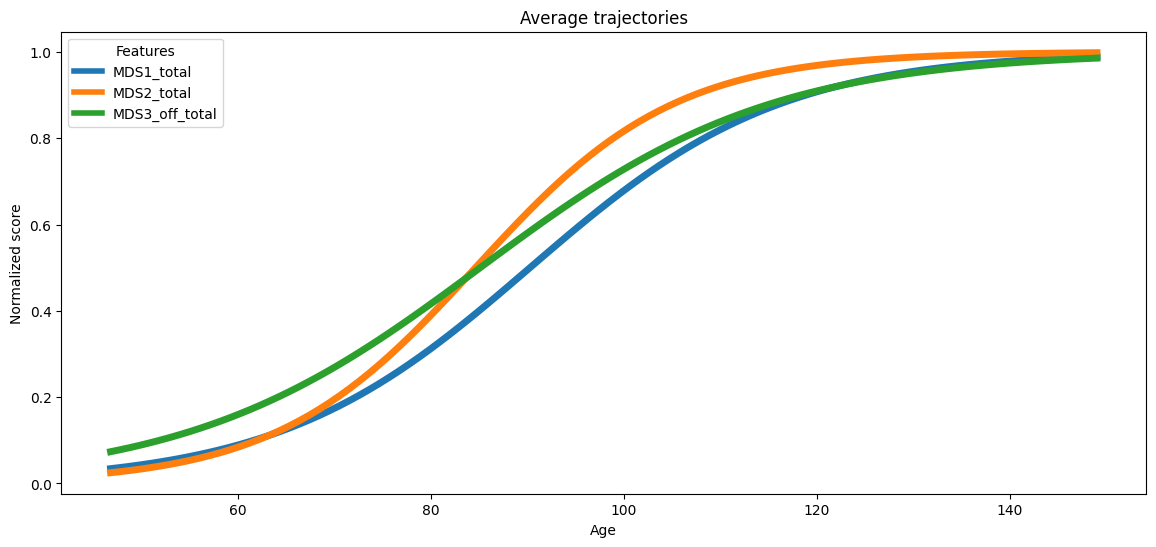
\includegraphics[width=0.41\textwidth]{figures/avg_example.png}
  \hfill
  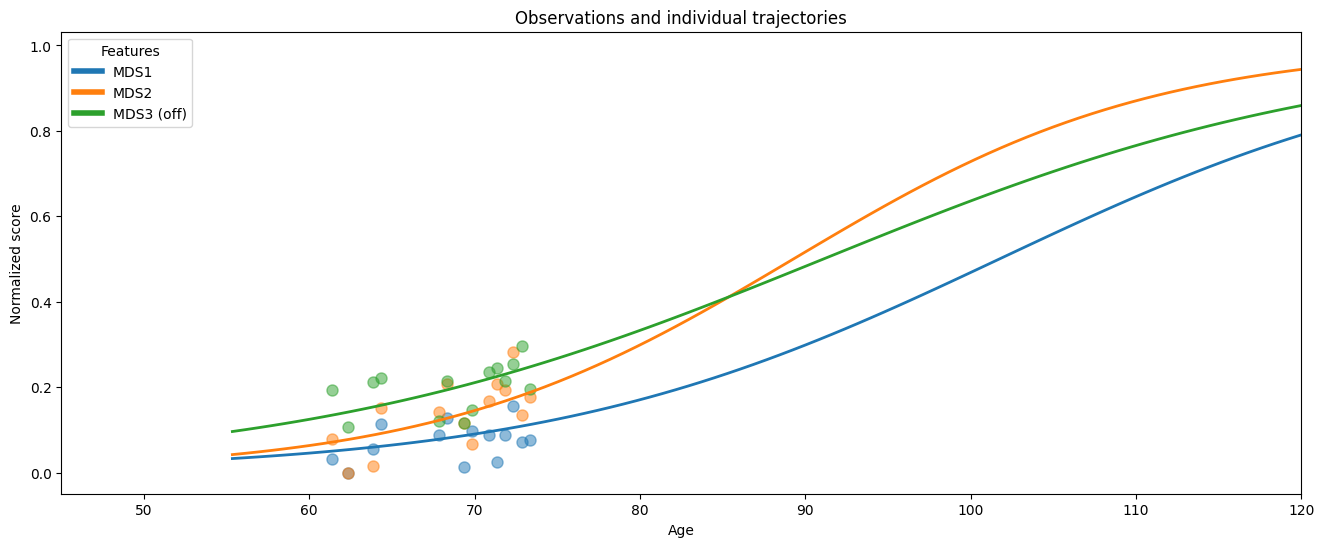
\includegraphics[width=0.48\textwidth]{figures/obs_example.png}
  \caption{Disease progression modeling with Leaspy on the built-in Parkinson's dataset. \textbf{Left:} Average population trajectory of clinical scores over the estimated disease timeline. \textbf{Right:} Personalized trajectory (solid line) and observed visits (dots) for one patient.}
  \label{fig:parkinson}
\end{figure}

%\paragraph{Alzheimer's disease (AD).} The AD Course Map~\cite{koval2021ad} uses Leaspy to create a spatiotemporal atlas of AD progression by jointly modeling neuropsychological and imaging data. It outperformed 56 competing methods in the TADPOLE open challenge and, when tested globally on over 4,600 patients, demonstrated the ability to enrich clinical trials with predicted progressors, reducing required sample sizes by up to 50\%~\cite{maheux2023forecasting}.

\paragraph{Alzheimer's disease (AD).} The AD Course Map~\cite{koval2021ad} uses Leaspy to create a spatiotemporal atlas of AD progression by jointly modeling neuropsychological assessments, the propagation of hypometabolism and cortical thinning across brain regions, and the deformation of the hippocampal shape. It outperformed 56 competing methods in the TADPOLE open challenge~\cite{marinescu2019tadpole} and, when tested globally on over 4,600 patients from ADNI, PharmaCog, and INSIGHT-preAD, demonstrated the ability to enrich clinical trials with predicted progressors, reducing required sample sizes by 38\% to 50\% depending on trial duration, outcome measure, and targeted disease stage~\cite{maheux2023forecasting}.


\paragraph{Huntington's disease.} Koval et al.\ applied the disease course mapping framework to identify the optimal intervention window for Huntington's disease clinical trials, demonstrating that the model could ``spot the time to treat'' by positioning patients on the disease timeline prior to symptom onset~\cite{koval2022forecasting}.

\paragraph{CADASIL.}
Kaisaridi et al.\ applied Leaspy to 395 patients from the French CADASIL referral center, modeling the joint progression of 14 clinical scores. Using a probabilistic mixture framework integrated into the MCMC-SAEM estimation procedure, they identified two clinically meaningful subtypes of disease progression: an early-onset, rapidly progressing group and a late-onset, slowly progressing group. This was achievedwithout resorting to post-hoc clustering, providing new insights into the heterogeneity of this rare cerebral small-vessel disease~\cite{kaisaridi2025mixture}.


\paragraph{Amyotrophic lateral sclerosis (ALS).}
The joint cause-specific spatiotemporal model~\cite{ortholand2025joint} was validated on data from the PRO-ACT dataset (over 2,100 ALS patients). The model jointly analyzes three ALSFRS-R subscales (bulbar, fine motor, gross motor) with competing events (non-invasive ventilation initiation and death) through a shared latent disease age. On a 10-fold cross-validation benchmark, the model achieved systematically better event discrimination (AUC, C-index) than the standard shared-random-effect joint model (JMbayes2), while using fewer parameters and avoiding the need for a precise reference onset time~\cite{ortholand2025joint}.

\subsubsection{Related approaches.}
Leaspy belongs to the broader family of data-driven disease progression models, a field that has developed rapidly since the early 2010s~\cite{oxtoby2023data,young2024data}. These methods can be organized along two axes: the type of data they require (cross-sectional vs.\ longitudinal) and whether they estimate a single disease timeline or multiple subtypes.

\paragraph{Cross-sectional models.} The Event-Based Model (EBM)~\cite{fonteijn2012event} and its discriminative variant (DEBM)~\cite{venkatraghavan2019disease} infer a cumulative sequence of biomarker abnormality events from a single visit per individual. While data-economical, they produce only discrete severity orderings and have limited forecasting utility without additional longitudinal information. The Subtype and Stage Inference algorithm (SuStaIn)~\cite{young2018uncovering} augments the EBM concept with unsupervised clustering, enabling joint subtyping and staging from cross-sectional data alone. SuStaIn has yielded high-impact results across Alzheimer's disease~\cite{vogel2021four}, multiple sclerosis~\cite{eshaghi2021identifying}, and other conditions, but does not model continuous biomarker trajectories.

\paragraph{Longitudinal models.} Several latent-time mixed-effects models have been proposed for continuous trajectory estimation. The Disease Progression Score (DPS)~\cite{jedynak2012computational} aligns biomarker data via a linear transformation of age into a disease score with sigmoid group-level dynamics; the Latent Time Joint Mixed Model (LTJMM)~\cite{li2019bayesian} extends this with a flexible Bayesian framework and covariate support. The Gaussian Process Progression Model (GPPM)~\cite{lorenzi2019probabilistic} offers a nonparametric alternative that avoids imposing parametric trajectory shapes but can be computationally expensive on large cohorts. SubLign~\cite{chen2022clustering} combines deep generative models with latent time-shifts for simultaneous subtyping and trajectory alignment using longitudinal data.

Compared to these approaches, Leaspy's Disease Course Mapping framework, introduced by Schiratti et al.~\cite{schiratti2017bayesian} and extended by Koval et al.~\cite{koval2021ad}, offers a distinctive combination of features: (i) a Riemannian geometric formulation that naturally handles bounded scores via logistic geodesics, (ii) interpretable individual-level random effects decomposed into time shift, acceleration, and inter-biomarker space shifts, (iii) a joint model linking longitudinal outcomes and competing survival events through a shared latent disease age~\cite{ortholand2025joint}, and (iv) a mixture extension for unsupervised subtyping~\cite{kaisaridi2025mixture}.

\newpage

\section{Motivation for Simulation Studies and Tools}

\subsection{The Role of Simulation in Statistical Methodology}

Simulation studies occupy a central position in the development and validation of statistical methods. Their fundamental advantage is epistemological: because the data-generating process is entirely under the experimenter's control, the true values of all parameters and latent quantities are known by construction. This makes it possible to evaluate estimator properties such as bias, variance, coverage of confidence intervals, sensitivity to model misspecification, that are inaccessible on real data, where a ground truth is never observed. As Morris, White and Crowther emphasize in their reference tutorial on the design, conduct and reporting of simulation studies~\cite{morris2019using}, this ability to compare estimates against a known truth is the defining strength of the simulation approach, and what distinguishes it from empirical benchmarks on real-world datasets.

Despite their power, simulation studies are often poorly designed, inadequately analyzed and incompletely reported, which can severely limit their scientific value and reproducibility. The ADEMP (Aims, Data-generating mechanisms, Estimands, Methods, and Performance measures) framework proposed by Morris et al.~\cite{morris2019using} provides a principled template for conducting and communicating such studies. This framework guided the simulation study reported in the original joint model paper~\cite{ortholand2025joint}, and it underpins the design choices made in the simulation tools developed in the present work.

Beyond methodological validation, simulated datasets present a practical advantage that is increasingly relevant in clinical research: they can be freely shared and distributed without the ethical, legal or privacy constraints that govern real patient data. A synthetic cohort generated under a calibrated model preserves the statistical properties of the original population (trajectory shapes, individual variability, censoring patterns) while containing no identifiable patient information. This makes simulated data a natural vehicle for reproducible research, open benchmarking, and collaborative method development across institutions.

\subsection{Importance in the Leaspy Context}

The combination of model complexity, data structure, and estimation challenges that characterizes the Leaspy framework makes simulation studies not merely useful, but methodologically indispensable. Several distinct considerations motivate this claim.

\paragraph{Absence of ground truth on real data.}
On real longitudinal cohorts such as PRO-ACT (ALS) or ADNI (Alzheimer's disease), the true individual random effects $(\tau_i, \xi_i, \mathbf{s}_i)$ are never observed. One can fit a model and obtain estimated parameters, but there is no external criterion against which to verify whether the estimates are biased, whether the posterior is well calibrated, or whether the algorithm has converged to the correct solution. Simulation is the only means to construct a controlled setting in which the estimator's output can be directly compared to a known truth, and thus the only means to quantify bias, mean squared error, and interval coverage.

\paragraph{Comparing personalization strategies without an oracle.}
Once the population model has been fitted, individual random effects are recovered via a \texttt{personalize} step that offers two algorithmic modes: a frequentist MAP estimate obtained by numerical optimization, and a Bayesian posterior estimate obtained by Gibbs sampling. These two approaches differ in computational cost, in the uncertainty information they return, and potentially in the accuracy of their point estimates. In clinical applications, biases in the estimated time shift $\hat{\tau}_i$ directly affect the positioning of each patient on the disease timeline, with consequences for trial enrichment, progression forecasting, and biomarker ordering analyses. Determining in which regimes each approach is preferable requires a ground truth that only simulation can supply.

\paragraph{Cases with sparse and heterogeneous data.}
Patients with neurodegenerative diseases often contribute a highly variable number of visits: some are followed for only two or three appointments, others for a decade or more, with irregular and patient-specific inter-visit intervals. This can lead to trajectories that are poorly identified from short follow-ups. In this regime of sparse observations, classical asymptotic guarantees such as consistency or normality of maximum likelihood estimators are not reliable guides to finite-sample behavior. Simulation provides the only principled way to explore how estimation quality degrades as the number of visits decreases, as visit spacing increases, or as individual heterogeneity grows.

\paragraph{Informative dropout and its interaction with the model.}
A pervasive challenge in neurodegenerative disease cohorts is informative dropout: patients who progress most rapidly are precisely those most likely to leave the study early, either because of disease severity, hospitalization, or death. This means that the absence of data is not random but is correlated with the unobserved latent state of the patient. Ignoring this mechanism leads to biased estimates of population parameters and individual trajectories. The joint model~\cite{ortholand2025joint} is specifically designed to address this problem by linking the longitudinal trajectory and the time-to-event process through a shared latent disease age, so that informative censoring is modeled rather than ignored. Simulation is the primary tool for verifying that the implementation of the joint simulation algorithm correctly reproduces this mechanism and for confirming that the estimation procedure remains approximately unbiased under this form of dependent censoring.

\paragraph{Non-linearity and Riemannian geometry.}
For standard linear models or generalized linear models, theoretical results guarantee consistency and asymptotic normality of maximum likelihood estimators under regularity conditions. In the spatiotemporal NLMEM framework of Leaspy, which operates on a product Riemannian manifold and involves intractable marginal likelihoods approximated by MCMC-SAEM, these guarantees are far harder to establish formally. Whether the algorithm converges to the correct fixed point, how many SAEM iterations are needed, and how sensitive the estimates are to initialization are all empirical questions that cannot be resolved analytically in the regime of real cohort sizes. Simulation studies allow these questions to be examined directly, under conditions that mirror the application setting.

\paragraph{Prerequisite for downstream statistical analyses.}
The individual parameters estimated by Leaspy will also be used as inputs to secondary analyses: variable selection, explainability methods, or predictive modeling applied to the personalized parameters $\hat{\tau}_i$, $\hat{\xi}_i$, and $\hat{\mathbf{s}}_i$. If these estimates are systematically biased or poorly calibrated, any downstream method, regardless of its own statistical validity, will inherit and propagate these errors, producing findings that cannot be reliably interpreted. Validating the estimation procedure through simulation is therefore a methodological prerequisite for any conclusion drawn from the individual parameters.

\subsection{Objectives of the Simulation Tools Developed in This Work}

The present work develops and integrates into the Leaspy codebase a set of simulation tools specifically designed for the joint model. These tools serve two complementary purposes.

The first is algorithmic: to provide a self-consistent and numerically robust implementation of the joint simulation procedure, extending the existing \texttt{simulate} method, currently restricted to the logistic model, to the joint model with its competing-events variant. This required extending the \texttt{estimate} method of the joint model to return event predictions compatible with the simulation pipeline, implementing inverse-transform sampling on the discrete visit grid, and handling the generalization to competing events through cause-specific conditional cumulative incidence functions.

The second is methodological: to enable rigorous simulation studies of the joint model, following the ADEMP framework \cite{morris2019using}. By generating synthetic cohorts under known model parameters, calibrated to real-world datasets such as PRO-ACT, these tools make it possible to evaluate the bias and coverage of MCMC-SAEM parameter estimates, to compare MAP and Gibbs personalization under varying data densities, and to quantify the effect of informative dropout on estimation. They also produce shareable, privacy-preserving synthetic datasets that can be distributed alongside the model code for reproducibility and benchmarking purposes.

\newpage

\section{Details on the Joint Model}

The joint model~\cite{ortholand2025joint} extends the Leaspy longitudinal framework to simultaneously model repeated clinical measurements and survival outcomes, without requiring a reliable reference time point. This is a key advantage in neurodegenerative disease contexts where disease onset is not directly observable.

The model is composed of three interconnected components. The longitudinal sub-model describes the evolution of a clinical score via a logistic trajectory parameterized by the latent disease age $\psi_i(t)$ (Equation~\eqref{eq:latent-age}), as already introduced in the main Leaspy framework. The survival sub-model describes the probability that patient $i$ survives beyond time $t$ using a Weibull distribution applied to the latent disease age:
\begin{equation}
  S_i(t) = S_0(\psi_i(t)) = \mathbf{1}_{\psi_i(t) > t_0}\, \exp\!\left(-\left(\frac{\psi_i(t) - t_0}{\nu}\right)^{\rho}\right) + \mathbf{1}_{\psi_i(t) \leq t_0},
\end{equation}
where $\nu > 0$ is a scale parameter and $\rho > 0$ is the shape parameter of the Weibull distribution; the model estimates the unconstrained reparametrisations $\tilde{\nu} = -\log\nu$ and $\tilde{\rho} = \log\rho$, which enforce positivity while enabling unconstrained optimisation. The linkage structure connecting the two sub-models is the shared latent disease age $\psi_i(t) = e^{\xi_i}(t - \tau_i) + t_0$, which encodes individual variability in disease onset ($\tau_i$) and progression rate ($e^{\xi_i}$). This differs from classical shared-random-effects joint models, which link the survival hazard to the value of the longitudinal outcome; here the link is structural, operating directly at the level of the disease timeline.

The formulation extends naturally to $L \geq 1$ competing events by assigning an independent pair of Weibull parameters $(\nu_l, \rho_l)$ to each event type $l \in \{1, \ldots, L\}$. In the single-event case the quantity of interest is the overall survival probability $S_i(t)$; in the competing-events case it becomes the set of cause-specific cumulative incidence functions $\mathrm{CIF}_{i,l}(t)$, each measuring the probability that event $l$ occurs by time $t$ in the presence of all other competing risks. When the longitudinal sub-model includes $K \geq 1$ latent sources $\mathbf{s}_i \in \mathbb{R}^K$, the survival sub-model is further coupled to the individual biomarker ordering pattern through a matrix of mixing weights $\boldsymbol{\zeta} \in \mathbb{R}^{K \times L}$. The survival shift $(\boldsymbol{\zeta}^\top \mathbf{s}_i)_l$ then enters an accelerated failure time reparametrization of the Weibull scale parameter for patient $i$ and event $l$:
\begin{equation}
  \nu_{i,l} = \nu_l \exp\!\left(-\xi_i - \frac{1}{\rho_l}\,(\boldsymbol{\zeta}^\top \mathbf{s}_i)_l\right),
  \label{eq:nu-rep}
\end{equation}
so that the individual biomarker ordering pattern encoded in $\mathbf{s}_i$ accelerates or decelerates the event-specific hazard beyond the shared disease pace $e^{\xi_i}$. The weight matrix $\boldsymbol{\zeta}$ is estimated jointly with all other fixed effects during the MCMC-SAEM fitting procedure. \\

\noindent The joint log-likelihood decomposes additively into longitudinal and survival data attachment terms plus prior attachment terms for both fixed and random effects, under the assumption that survival and longitudinal processes are conditionally independent given the latent random effects~\cite{rizopoulos2012joint}. \\
 
\noindent Estimation proceeds via the MCMC-SAEM algorithm, initialized from a pre-trained longitudinal model and a Weibull Accelerated Failure Time (AFT) survival model. The algorithm runs for a burn-in phase followed by a Robbins-Monro convergence phase to extract posterior means of the fixed effects. Individual random effects $(\tau_i, \xi_i)$ are personalized in a second step by maximizing the posterior likelihood given each patient's observations and censored event time, using \texttt{scipy.optimize.minimize}. \\

\noindent The joint model was validated on simulated data following the ADEMP framework~\cite{morris2019using}. Using $M = 100$ datasets of $N = 200$ patients each, generated under the model's own structure with ALS-calibrated parameters, the estimation procedure recovered the true model parameters with low relative bias (under 5\% for most parameters) and accurate coverage rates. Individual random effects were also recovered reliably, with high intraclass correlations between estimated and true values. Benchmarked against four reference models on real ALS data from the PRO-ACT dataset, an AFT survival model, the standalone longitudinal model, a two-stage model, and a shared-random-effects joint model (JMbayes2), the joint model achieved superior or comparable predictive and discriminative performance while using fewer parameters. Full details of the simulation study and benchmark results are reported in~\cite{ortholand2025joint}.

\newpage 

\section{The Joint Simulation Algorithm}

\subsection{The Original Algorithm}

In the original article describing the joint model~\cite{ortholand2025joint}, the simulation of synthetic patient cohorts under the joint model proceeds in six sequential steps, described below. 

\begin{enumerate}
  \item \textbf{Simulate individual random effects}. For each patient, draw the log-acceleration factor $\xi_i$ and time shift $\tau_i$ independently from their population distributions: $\xi_i \sim \mathcal{N}(0,\, \sigma_\xi^2), \quad
  \tau_i \sim \mathcal{N}(t_0,\, \sigma_\tau^2)$.
  \item \textbf{Simulate age at first visit}. The age at first visit is drawn as $t_{i,0} = \tau_i + \delta_{f_i}$, where $\delta_{f_i} \sim \mathcal{N}(\bar{\delta}_f, \sigma_{\delta_f}^2)$ is a random offset relative to the patient's estimated disease onset. 
  \item \textbf{Simulate visit schedule}. Inter-visit intervals $\delta_{v_{i,j}} \sim \mathcal{N}(\bar{\delta}_v, \sigma_{\delta_v}^2)$ and a total follow-up duration $T_{f_i} \sim \mathcal{N}(\overline{T_f}, \sigma_{T_f}^2)$ determine the visit times $t_{i,0} < t_{i,1} < \cdots < t_{i,n_i}$, where $n_i$ is the number of visits satisfying $t_{i,j} \leq t_{i,0} + T_{f_i}$.
  \item \textbf{Simulate longitudinal outcomes}. The latent disease age $\psi_i(t_{i,j})$ is computed for each visit. The expected outcome value is then $\gamma_0(\psi_i(t_{i,j}))$ as defined by the logistic trajectory. Observed outcomes are sampled with additive noise; in the simulation study, a Beta distribution with mode $\gamma_0(\psi_i(t_{i,j}))$ and concentration $p$ is used to match the bounded nature of clinical scores: $y_{i,j} \sim \mathcal{B}(\gamma_0(\psi_i(t_{i,j})), p)$.
  \item \textbf{Simulate event times}. The event time $T_{e_i}$ is drawn from the Weibull survival distribution implied by the latent disease age. Using the inverse-transform method, this is equivalent to: $T_{e_i} \sim e^{-\xi_i}\, \mathcal{W}(\nu, \rho) + \tau_i$, where $\mathcal{W}(\nu, \rho)$ denotes the Weibull distribution with scale $\nu$ and shape $\rho$.
  \item \textbf{Apply censoring}. The event time and visit schedule are reconciled by applying two censoring rules: (i) all visits occurring after the event ($t_{i,j} > T_{e_i}$) are removed from the follow-up; (ii) events occurring after the last remaining visit ($T_{e_i} > t_{i,\max(j)}$) are treated as right-censored. This produces the observed tuple $(y_{i,j}, T_{e_i}, B^e_i)$, where the censoring indicator $B^e_i = 1$ if the event was observed and $B^e_i = 0$ if it was censored.
\end{enumerate}

The simulation algorithm relies on two disjoint sets of parameters. The model parameters, read directly from the fitted joint model, are: the population distributions of the individual random effects ($t_0$, $\sigma_\tau$, $\sigma_\xi$), the Weibull survival parameters ($\nu$, $\rho$), and the source-to-survival mixing weights $\zeta$ whenever the model includes latent sources. These parameters are set once and for all during model fitting and are not accessible to the user at simulation time. The study parameters, supplied by the user, govern the structure of the synthetic cohort: the number of patients $N$, the mean and standard deviation of the first-visit offset from disease onset ($\bar{\delta}_f$, $\sigma_{\delta_f}$), the mean and standard deviation of the per-patient follow-up duration ($\overline{T_f}$, $\sigma_{T_f}$), and the mean and standard deviation of inter-visit intervals ($\bar{\delta}_v$, $\sigma_{\delta_v}$). An additional technical parameter, \texttt{min\_spacing\_between\_visits}, enforces a minimum gap between successive visits and prevents numerical artefacts from excessively close observations.

\subsection{Adaptations in the Leaspy Implementation}

The Leaspy implementation follows the six-step procedure above and introduces the following adaptations.

\paragraph{Visit schedule modes.}
The implementation supports two distinct visit generation modes. In the \textit{random} mode, the visit schedule is generated stochastically following steps~2 and~3 above, driven by the study parameters supplied by the user. In the \textit{dataframe} mode, the user instead provides an explicit DataFrame specifying each patient's identifier and visit times directly, bypassing steps~2 and~3 entirely. Individual parameters are then sampled from the fitted population distributions for each patient listed in the DataFrame, in the order they appear.

\paragraph{Data driven estimation of study parameters.}
As an extension developed in this work, when the user does not supply some or all study parameters for the \textit{random} mode, they can instead provide a dataset, usually the same dataset used to fit the model. In that case, the missing parameters are estimated automatically from the observed visit process. Specifically, $\bar{\delta}_f$ is set to zero by construction, since the empirical mean of centered first-visit ages is zero by definition; $\sigma_{\delta_f}$ is taken as the empirical standard deviation of observed first-visit ages across patients, which serves as a proxy for the dispersion of the first-visit offset from disease onset, given that the individual disease onsets $\tau_i$ are not directly observable. The parameters $\overline{T_f}$ and $\sigma_{T_f}$ are obtained from the empirical distribution of per-patient follow-up durations (last minus first visit), and $\bar{\delta}_v$ and $\sigma_{\delta_v}$ are estimated from the distribution of all observed inter-visit gaps. This feature is not present in the base simulation algorithm of Leaspy for the logistic model; it introduces a dependency on the training data and breaks the strict separation between the generative mechanism and the observed sample, which should be kept in mind when interpreting simulation results.

\paragraph{Standardization of latent sources.}
When the model includes latent sources ($K \geq 1$), the source components $s_{i,k}$ for each dimension $k$ are first drawn independently from $\mathcal{N}(0, 1)$ and then standardized across the simulated cohort: each source dimension is empirically recentered and rescaled to unit variance. This ensures that the sources are approximately orthogonal to the mean in finite samples, reproducing the centering constraint that is imposed during model fitting.

\paragraph{Event time sampling via the adapted \texttt{estimate} method.}
A key contribution of this work is the extension of the joint model's \texttt{estimate} method to return event predictions alongside longitudinal trajectories, and its integration into the simulation pipeline. The original algorithm samples event times directly from the closed-form Weibull formula $T_{e_i} \sim e^{-\xi_i}\,\mathcal{W}(\nu, \rho) + \tau_i$. The implementation instead reuses the model's own \texttt{estimate} method, which evaluates the individual trajectory at each planned visit time $t_{i,j}$ and returns a conditional quantity: for a single-event model it returns the conditional survival $S_i(t_{i,j})/S_i(t_{i,0})$, and for competing events it returns the conditional cause-specific cumulative incidence functions $\text{CIF}_{i,l}(t_{i,j})/S_i(t_{i,0})$, each conditioned on the patient being alive at the first planned visit $t_{i,0}$. From these, the total conditional cumulative distribution function is assembled as:
\begin{equation}
F_i^{\,\text{cond}}(t_{i,j}) = 
\begin{cases}
1 - S_i(t_{i,j})\,/\,S_i(t_{i,0}) & \text{(single event),} \\[4pt]
\displaystyle\sum_{l=1}^{L} \text{CIF}_{i,l}(t_{i,j})\,/\,S_i(t_{i,0}) & \text{(competing events).}
\end{cases}
\end{equation}
Inverse-transform sampling is then applied on this discrete grid: a uniform draw $U \sim \mathcal{U}[0,1]$ is compared to $F_i^{\,\text{cond}}$ at each visit, and the event time is set to the first visit time $t_{i,j}$ at which $F_i^{\,\text{cond}}(t_{i,j}) \geq U$. If $U$ exceeds the total conditional CDF at the last planned visit, the patient is right censored at that visit.

Two consequences follow from this design. First, because the CDF is evaluated only at the planned visit times, event times are constrained to lie on the visit grid rather than being continuous. Second, because the sampling is conditioned on survival at $t_{i,0}$, the event can never be placed before the first planned visit.

\paragraph{Beta noise with variance clamping.}
Longitudinal outcomes are sampled from a Beta distribution with mean $\mu = \gamma_0(\psi_i(t_{i,j}))$ and variance $\sigma^2$ taken from the fitted noise model. A Beta distribution with mean $\mu$ is only well defined when $\sigma^2 < \mu(1 - \mu)$; this constraint can be violated when the trajectory approaches 0 or 1, that is when the patient is near the floor or ceiling of a clinical score. In such cases the implementation clamps the variance to $0.99\,\mu(1-\mu)$ and emits a warning identifying the affected patient, visit time, and feature.

\paragraph{Censoring after rounding.}
The minimum visit spacing filter operates by rounding visit times to the decimal precision compatible with \texttt{min\_spacing\_between\_visits} and removing duplicate time points. Because rounding can advance a visit time beyond the event time, a final censoring pass is applied after rounding: any visit whose rounded time exceeds the patient's event time is removed from the dataset. This step is not part of the original six-step procedure but is required by the discrete-grid implementation to preserve the constraint that all longitudinal observations precede the event.

\paragraph{Generalization to competing events.}
In the single-event case the event indicator is set to 1 whenever the event time falls within the follow-up window. In the competing-events case ($L > 1$), the event type $l^*$ is drawn at the identified visit time by treating the incremental cause-specific CIF as unnormalized probabilities:
\begin{equation}
p(l^* = l) \;\propto\; \max\left(\text{CIF}_{i,l}(t_{i,j}) - \text{CIF}_{i,l}(t_{i,j-1}),\; 0\right),
\end{equation}
and the censoring indicator is set to $B^e_i = l^*$, following the convention that $B^e_i = 0$ denotes censoring and $B^e_i = l$ denotes cause-$l$ event.

\paragraph{Test coverage in the library.}
The implementation is accompanied by unit and functional tests integrated into the Leaspy test suite. On the simulation side, two unit tests cover the \texttt{JointSimulationAlgorithm}: one verifies the \textit{random} visit mode by checking that the output dataset is non-empty, contains the expected number of patients, and that visit times are strictly increasing within each individual; the other verifies the \textit{dataframe} visit mode by checking that all simulated visits belong to the user-supplied input schedule (the algorithm may drop visits after a simulated event, but must not introduce new time points) and that all model features are present in the output. On the \texttt{estimate} method side, four functional tests cover the extended joint model behaviour: one checks numerical correctness of the returned values for a univariate model against hardcoded expectations; one verifies that \texttt{to\_dataframe=True} produces a \texttt{DataFrame} with columns \texttt{model.features + model.event\_features} whose values are consistent with the raw dictionary output; one checks that passing a \texttt{pd.MultiIndex} as timepoints automatically activates the DataFrame output mode and preserves the original index ordering; and one tests the multivariate case, verifying that the output shape is $(n_{\text{tpts}},\, n_{\text{features}} + L)$ where $L$ is the number of events.

\newpage

\section{Validation and Results}

\subsection{Method of Evaluation}

\subsubsection{Principle}

The evaluation rests on a simulation-based identification scheme whose conceptual core is the following: if a model is correctly specified and its estimation procedure is consistent, then fitting the model on data generated by that same model under known parameters must recover those parameters. This self-consistency requirement is the most demanding test one can impose on a complex generative pipeline, because it simultaneously exercises the simulation algorithm, the likelihood implementation, and the numerical estimation procedure. The triangular structure of the evaluation, from reference model to synthetic cohort to re-estimated model, makes it possible to verify that the model truly encodes, in its generative mechanism, the same statistical structure it learns during fitting.
The procedure unfolds in three sequential stages, summarised in Figure~\ref{fig:eval-principle}.

\begin{enumerate}
  \item \textbf{Reference model.} A reference parameter vector $\theta^{*}$ is defined, either by fitting the joint model on a real dataset or by setting it to a synthetic ground truth. This reference model serves as the source of truth for all subsequent comparisons.
  \item \textbf{Repeated simulation and re-estimation.} A total of $M$ synthetic cohorts are generated by the joint simulation algorithm under the reference model parameters $\theta^{*}$. Each synthetic cohort is then fitted from scratch using the same MCMC-SAEM procedure, yielding $M$ estimated parameter vectors $\hat{\theta}^{(m)}$. Individual random effects are also recovered for each synthetic patient and compared to the true values used to generate the data.
  \item \textbf{Comparison.} The $M$ estimated parameter vectors $\hat{\theta}^{(m)}$ are compared component-wise to $\theta^{*}$ through the scalar performance measures described in Section~\ref{sec:metrics}. The $N \times M$ pairs of true and estimated individual random effects are assessed through agreement statistics that distinguish systematic bias from random variability.
\end{enumerate} 

The diagnostic force of this design lies precisely in its circularity. The simulated data are not drawn from an independent external process: they are direct realisations of the model being validated. If the simulation algorithm correctly implements the joint model structure, and if the estimation procedure is consistent, then the estimated parameters must converge to the true ones as $N$ and $M$ grow. A persistent bias in $\hat{\theta}^{(m)}$, or a low intraclass correlation between estimated and true individual parameters, therefore constitutes evidence of an inconsistency between the generative mechanism and the likelihood, an identifiability failure at the chosen sample size, or a numerical artefact in the optimisation. This makes simulation-based self-consistency the primary instrument for verifying that the joint model not only fits real data but genuinely represents the underlying generative process.

\begin{figure}[htbp] 
  \centering
  \resizebox{\linewidth}{!}{%
  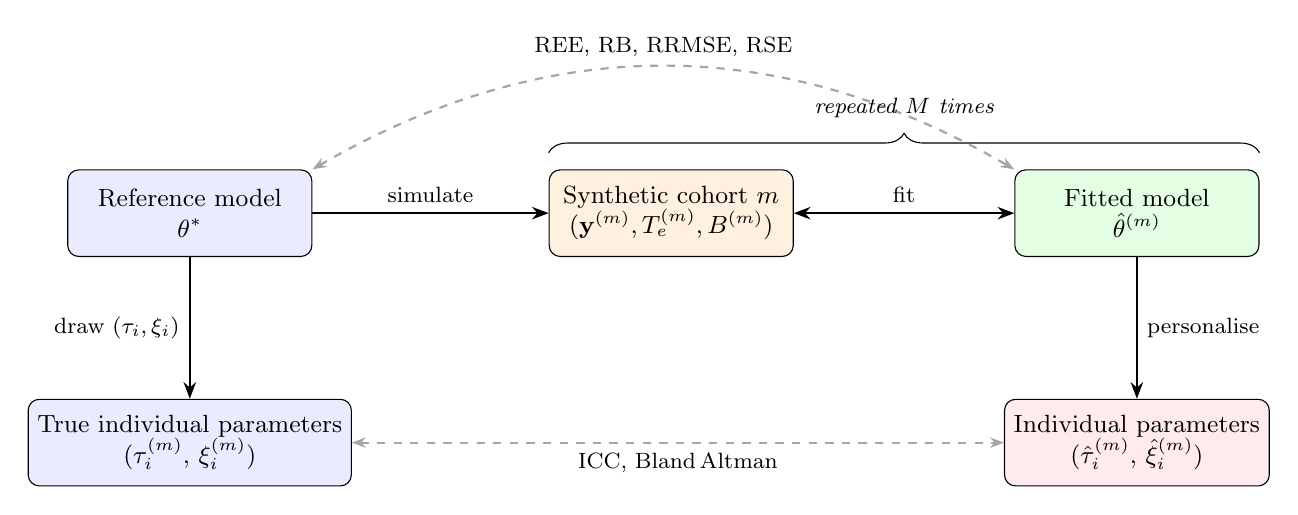
\begin{tikzpicture}[
      node distance = 1.4cm and 2.0cm,
      box/.style    = {rectangle, draw, rounded corners=4pt,
                       minimum width=3.1cm, minimum height=1.1cm,
                       align=center, font=\small},
      arr/.style    = {-{Stealth[length=6pt]}, thick},
      darr/.style   = {{Stealth[length=5pt]}-{Stealth[length=5pt]},
                       dashed, thick, color=gray!70},
    ]
    \node[box, fill=blue!8]     (ref) {Reference model\\$\theta^{*}$};
    \node[box, fill=orange!12,  right=3.0cm of ref] (sim)
          {Synthetic cohort $m$\\$(\mathbf{y}^{(m)}, T_e^{(m)}, B^{(m)})$};
    \node[box, fill=green!10,   right=2.8cm of sim] (fit)
          {Fitted model\\$\hat{\theta}^{(m)}$};
    \node[box, fill=red!8,      below=1.8cm of fit] (per)
          {Individual parameters\\$(\hat{\tau}_i^{(m)},\,\hat{\xi}_i^{(m)})$};

    % True individual parameters node
    \node[box, fill=blue!8,    below=1.8cm of ref] (trueip)
          {True individual parameters\\$(\tau_i^{(m)},\,\xi_i^{(m)})$};

    % Flow arrows 
    \draw[arr] (ref)  -- node[above, font=\footnotesize]{simulate} (sim);
    \draw[{Stealth[length=6pt]}-{Stealth[length=6pt]}, thick] (sim) -- node[above, font=\footnotesize]{fit} (fit);
    \draw[arr] (fit)  -- node[right, font=\footnotesize]{personalise} (per);
    \draw[arr] (ref.south) -- node[left, font=\footnotesize]{draw $(\tau_i, \xi_i)$} (trueip);

    % Comparison arrows
    \draw[darr] (ref.north east) to[out=30, in=150] node[above, font=\footnotesize, color=black] 
          {REE, RB, RRMSE, RSE} (fit.north west);
    \draw[darr] (trueip.east) -- node[below, font=\footnotesize, color=black]
          {ICC, Bland\,Altman} (per.west);

    % Repetition brace
    \draw[decorate, decoration={brace, amplitude=7pt, raise=6pt}]
          (sim.north west) -- (fit.north east)
          node[midway, above=15pt, font=\footnotesize\itshape]
               {repeated $M$ times};
  \end{tikzpicture}}%
  \caption{Schematic of the simulation-based evaluation pipeline. The reference model with fixed parameters $\theta^{*}$ generates $M$ synthetic cohorts; for each cohort, a fresh model is fitted and then personalised.}
  \label{fig:eval-principle}
\end{figure}

\subsubsection{Metrics}
\label{sec:metrics}

Two families of performance measures are used, corresponding to the two levels of inference in the joint model: population fixed effects and individual random effects.

\paragraph{Population parameter recovery.}
Let $\theta \in \mathbb{R}$ denote a scalar estimand, a single component of $\theta^{*}$, and let $\hat{\theta}^{(m)}$ be its estimate from repetition $m$, for $m = 1, \ldots, M$. All relative quantities below are expressed as percentages when they derive from REE.

The {Relative Estimation Error} for repetition $m$ is:
\begin{equation}
  \mathrm{REE}(m) = \frac{\hat{\theta}^{(m)} - \theta}{|\theta|} \times 100,
\end{equation}
and measures the signed percentage deviation of a single estimate from the true value. Its distribution across repetitions reflects the full sampling behaviour of the estimator at sample size $N$.

The {Relative Bias} (RB) is the mean REE over all repetitions:
\begin{equation}
  \mathrm{RB}(\hat{\theta}) = \frac{1}{M}\sum_{m=1}^{M} \mathrm{REE}(m),
\end{equation}
and quantifies the systematic tendency of the estimator to over- or under-estimate $\theta$ across repeated datasets of the same size.

The {Relative Root Mean Squared Error} (RRMSE) combines bias and variance into a single scalar:
\begin{equation}
  \mathrm{RRMSE}(\hat{\theta}) = \sqrt{\frac{1}{M}\sum_{m=1}^{M} \mathrm{REE}(m)^2}.
\end{equation}
It reduces to RB when the estimator is unbiased, and always satisfies $\mathrm{RRMSE} \geq |\mathrm{RB}|$, so any excess of RRMSE over $|\mathrm{RB}|$ is attributable to Monte Carlo variability.

The {Empirical Relative Standard Error} (RSE) measures the variability of the estimator relative to its own mean, independently of the true value:
\begin{equation}
  \mathrm{RSE}(\hat{\theta})
  = \frac{\mathrm{SE}_{\mathrm{emp}}(\hat{\theta})}{|\bar{\hat{\theta}}|},
  \qquad
  \mathrm{SE}_{\mathrm{emp}}(\hat{\theta})
  = \sqrt{\frac{\displaystyle\sum_{m=1}^{M}\bigl(\hat{\theta}^{(m)} - \bar{\hat{\theta}}\bigr)^2}{M - 1}},
\end{equation}
where $\bar{\hat{\theta}} = M^{-1}\sum_m \hat{\theta}^{(m)}$. The RSE is a dimensionless coefficient of variation for the estimator: values close to zero indicate a stable estimator whose output changes little from one synthetic cohort to the next, while large values indicate that the estimation is sensitive to the particular realization of the data.

\paragraph{Individual random effect recovery.}
Once the population parameters are estimated, individual random effects $(\hat{\tau}_i, \hat{\xi}_i)$ are recovered by personalisation. Because the true values $(\tau_i, \xi_i)$ are known by construction, their accuracy is assessed through two complementary tools.

The {Intraclass Correlation Coefficient} ICC(3,1), defined under the two-way mixed-effects model with $k = 2$ raters and absolute agreement, is:
\begin{equation}
  \mathrm{ICC}(3,1) = \frac{MS_B - MS_E}{MS_B + (k - 1)\,MS_E}, \quad k = 2,
\end{equation}
where $MS_B$ is the mean square between subjects and $MS_E$ is the mean square error, computed from the matrix whose two columns are the true and estimated values. The ICC(3,1) is the preferred agreement statistic here rather than the Pearson correlation, because Pearson's $r$ is invariant to linear rescaling: an estimator that correctly ranks individuals but applies a systematic affine shift would obtain a high $r$ while still being practically misleading. The ICC(3,1) penalises both lack of correlation and systematic offset, so that an ICC of 1 indicates exact pointwise agreement, an ICC near 0 indicates agreement no better than chance, and negative values reveal a systematic disagreement that is worse than ignoring the model entirely. Reporting ICC(3,1) alongside Pearson's $r$ therefore makes it possible to distinguish a correctly ordered but shifted estimator from one that achieves genuine agreement.

The {Bland-Altman analysis} provides a graphical complement to the ICC. For each individual $i$ and each repetition $m$, the difference $\hat{\theta}_i^{(m)} - \theta_i^{(m)}$ is plotted against the mean $(\hat{\theta}_i^{(m)} + \theta_i^{(m)})/2$, pooled across all $M$ repetitions. Three summary quantities are reported: the bias (mean difference), which reveals any constant over- or under-estimation; the limits of agreement $\pm 1.96\,\mathrm{SD}$, which delimit the interval capturing approximately 95\% of individual differences; and the dependence of the difference on the mean, which would indicate proportional bias. A narrow symmetric band centred on zero is the signature of an accurate and unbiased personalisation procedure.
 
\subsection{Experimental Setup}

The reference model $\theta^*$ is a joint model fitted on the PULSE dataset, with a single event ($L = 1$). The simulation study is carried out in the \textit{random} visit mode with the following study parameters: first-visit offset $\bar{\delta}_f = -2.0$ years and $\sigma_{\delta_f} = 1.0$ year; follow-up duration $\overline{T_f} = 6.0$ years and $\sigma_{T_f} = 2.0$ years; inter-visit interval $\bar{\delta}_v = 0.083$ years and $\sigma_{\delta_v} = 0.042$ years; and a minimum spacing between visits of $0.05$ years. These parameters are deliberately chosen to place each simulated cohort in favourable conditions: the short inter-visit interval and long follow-up produce a dense observation schedule, so that each patient contributes many data points. This abundance of information per individual reduces the number of MCMC-SAEM iterations required to reach convergence both at the fitting and at the personalisation stage. 

Each synthetic cohort contains $N = 500$ patients, and the experiment is repeated $M = 50$ times. Each fresh model is fitted using the MCMC-SAEM algorithm with $N_{\mathrm{iter}} = 30000$ iterations, and the subsequent personalisation step runs for $N_{\mathrm{perso}} = 5000$ iterations. Naturally, the computational cost of this procedure is substantial, as it requires fitting $M$ separate joint models from scratch. Better results could be obtained by increasing $N$ and $M$, but this would further increase the computational burden. The chosen values of $N$ and $M$ represent a compromise between statistical power and practical feasibility, while still providing a robust assessment of the model's self-consistency.


\subsection{Results and Interpretation}
The results of the simulation study are summarised in Table~\ref{tab:population_recovery} for population parameters. The distributions of the Relative Estimation Error across the $M$ repetitions are displayed in Figure~\ref{fig:ree_all}, while the quality of individual parameter recovery is examined in detail through the scatter plots of Figure~\ref{fig:param_comparison} and the Bland-Altman plots of Figure~\ref{fig:bland-altman}. 

\subsubsection{Population parameter recovery}

Before turning to the numerical results, two parameters require special treatment: the mixing coefficient matrix $\beta$ and the source-to-survival coupling matrix $\boldsymbol{\zeta}$. As introduced in the mathematical background in section \ref{sec:math-background}, the space shifts are defined as $\mathbf{w}_i = \mathbf{A}\mathbf{s}_i$, where the columns of the mixing matrix $\mathbf{A}$ are constructed from the free coefficients $\beta$, and the survival shifts entering the Weibull reparametrisation \eqref{eq:nu-rep} are $(\boldsymbol{\zeta}^\top \mathbf{s}_i)_l$. Both quantities are linear in the latent sources $\mathbf{s}_i$, and are therefore invariant under any rotation $R \in \mathrm{O}(K)$ of the source space: replacing $\mathbf{s}_i \to R\mathbf{s}_i$, $\mathbf{A} \to \mathbf{A}R^\top$, and $\boldsymbol{\zeta} \to R\boldsymbol{\zeta}$ leaves all model predictions, and hence the entire likelihood, unchanged. As a consequence, individual components of $\beta$ and $\boldsymbol{\zeta}$ are not separately identifiable: they can vary arbitrarily across simulation repetitions through orthogonal rotations of the source space without any modification to the data attachment. Reporting component-wise REE for these parameters is therefore meaningless. The quantities that are invariant to such rotations are the Frobenius norm $\|\beta\|_F$ for the mixing matrix, since Frobenius norm is unitarily invariant, and the Euclidean norm $\|\boldsymbol{\zeta}\|$ for the coupling vector. These scalar summaries are the estimands reported in Table~\ref{tab:population_recovery}.

Table~\ref{tab:population_recovery} and Figure~\ref{fig:ree_all} display the performance measures for all population parameters, grouped by quality of recovery. The parameters most accurately recovered are those governing the average disease trajectory and its longitudinal variability. The reference disease time $t_0$ achieves a relative bias of $-0.13\%$ and an RRMSE of $0.94\%$, the lowest of all scalar parameters. This exceptional precision reflects the fact that $t_0$ is identified as the central tendency of all individual time-shift distributions simultaneously: with $N$ patients each contributing several longitudinal observations, the effective sample size for this estimand is very large and finite-sample fluctuations are effectively averaged out. The observation noise standard deviation $\sigma$ is similarly well identified ($\mathrm{RB} = -4.19\%$, $\mathrm{RRMSE} = 4.19\%$, $\mathrm{RSE} = 0.002$), because it is estimated from within-patient residuals across the entire dataset and its RSE is the smallest of all reported parameters, reflecting negligible repetition-to-repetition variability. The mean log-initial position $\tilde{g}$ is recovered with $\mathrm{RB} = -3.70\%$ and $\mathrm{RRMSE} = 4.24\%$: with dense observations, the sigmoidal trajectory shape tightly constrains the plateau levels of each clinical score. The inter-individual time-shift dispersion $\sigma_\tau$ is recovered with modest bias ($\mathrm{RB} = -4.18\%$) and slightly larger RRMSE ($5.69\%$), as between-subject spread requires aggregating information across individuals rather than across visits. Finally, the Frobenius norm $\|\beta\|_F$ is well recovered ($\mathrm{RB} = +2.33\%$, $\mathrm{RRMSE} = 3.87\%$), confirming that the total energy of the space-shift representation is consistently estimable even though the orientation of $\beta$ in source space is not identifiable.

The mean log-progression speed $\tilde{v}_0$ and the Weibull shape parameter $\tilde{\rho}$ both exhibit relative biases of approximately $-18\%$ and RRMSEs in the range $18$--$23\%$. The systematic underestimation of $\tilde{v}_0$ is partly structural. This parameter controls the shared disease progression speed and enters the latent disease age $\psi_i(t)$ multiplicatively with $e^{\xi_i}$. During the MCMC-SAEM iterations, the centering operation applied to $\xi_i$ transfers any residual drift of the empirical mean of $\xi$ into an update of $\log v_0$ in the opposite direction. In finite samples, this centering is imperfect and the resulting drift propagates as a persistent downward bias in $\tilde{v}_0$. For $\tilde{\rho}$, the shape of the Weibull hazard is identified exclusively from the temporal distribution of observed events and censoring patterns. With only one event per patient and a censoring fraction that depends on follow-up duration, the effective statistical information about the hazard shape is limited; the corresponding RSE of $0.188$ is the largest among all parameters except $\|\boldsymbol{\zeta}\|$, indicating substantial repetition-to-repetition variability that compounds the systematic underestimation visible in Figure~\ref{fig:ree_all}.

The parameters estimated with the greatest difficulty are $\sigma_\xi$, $\tilde{\nu}$, and $\|\boldsymbol{\zeta}\|$. The log-acceleration standard deviation $\sigma_\xi$ is the most severely biased parameter in the study, with $\mathrm{RB} = +49.16\%$ and $\mathrm{RRMSE} = 49.56\%$, corresponding to a systematic overestimation. Two distinct mechanisms contribute to this bias. First, in the logistic model, the log-acceleration $\xi_i$ and the time shift $\tau_i$ are only partially separated by the data: a patient who progresses rapidly (large positive $\xi_i$) and one who had an early onset (small $\tau_i$) produce similar longitudinal observations over a finite follow-up window. Part of the temporal heterogeneity that is truly due to $\tau_i$ is therefore absorbed into $\xi_i$ by the estimation procedure, inflating the recovered variance. Second, the M-step estimate of $\sigma_\xi^2$ aggregates the posterior second moments of all $\xi_i$, and these posterior second moments include irreducible posterior uncertainty in addition to genuine inter-individual variance. This posterior inflation effect is attenuated but not eliminated when longitudinal data are dense. Notably, the RSE of $\sigma_\xi$ is only $0.043$, comparable to those of well-recovered parameters: the overestimation is stable and systematic across repetitions rather than being driven by occasional outlier simulations, as confirmed by the tightly located box in Figure~\ref{fig:ree_all}.

The Weibull scale parameter $\tilde{\nu}$ is overestimated by $-35.72\%$ in relative terms. This bias is directly linked to the overestimation of $\sigma_\xi$ through the identifiability constraint implemented in the MCMC-SAEM centering step, which simultaneously adjusts $\log v_0$, $\xi_i$, and $n\_\log\_\nu$ by the empirical mean of the current $\xi$ realizations. When $\sigma_\xi$ is overestimated, the empirical spread of $\xi_i$ is inflated, and the resulting centering shift is amplified, propagating a systematic negative shift into $n\_\log\_\nu = -\log\nu$. The two biases are therefore not independent: the joint misestimation of $(\sigma_\xi, \tilde{\nu})$ reflects a single underlying confounding between inter-individual progression speed variability and the Weibull time scale.

Finally, $\|\boldsymbol{\zeta}\|$ presents a contrasting profile: its mean relative bias is only $+6.08\%$, but its RRMSE reaches $38.23\%$ and its RSE of $0.359$ is by far the largest of all reported parameters. This dissociation between low mean bias and high variability reflects the nature of $\boldsymbol{\zeta}$ as a second-order coupling parameter. It modulates the influence of individual biomarker ordering patterns $\mathbf{s}_i$ on the event-specific hazard through the survival shift $(\boldsymbol{\zeta}^\top \mathbf{s}_i)_l$. When the true coupling is weak, as in the reference model ($\|\boldsymbol{\zeta}\|^* = 0.481$), the likelihood surface in the direction of $\boldsymbol{\zeta}$ is nearly flat, and the optimizer converges to different local solutions across repetitions without materially changing the data attachment. The norm $\|\boldsymbol{\zeta}\|$ is recoverable on average, but its estimate is highly volatile at the level of individual simulations, suggesting that this parameter is close to the practical limit of identifiability at the considered sample size.

\begin{table}[htbp]
\centering
\caption{Population parameter recovery metrics.}
\label{tab:population_recovery}
\begin{tabular}{lrrrrr}

Parameter & $\theta^{*}$ (reference)& $\bar{\hat{\theta}}$ (estimate)& RB (\%) & RRMSE (\%) & RSE \\
\hline        
$t_0$                    & $66.079$ & $65.992$ & $-0.13$ & $0.94$ & $0.010$ \\
$\sigma$                 & $0.391$  & $0.375$  & $-4.19$ & $4.19$ & $0.002$ \\
$\tilde{g}$ (mean)       & $0.499$  & $0.480$  & $-3.70$ & $4.24$ & $0.022$ \\
$\sigma_{\tau}$          & $10.363$ & $9.931$  & $-4.18$ & $5.69$ & $0.041$ \\
$\|\beta\|_F$            & $0.305$  & $0.312$  & $+2.33$ & $3.87$ & $0.031$ \\
$\tilde{v}_0$ (mean)     & $-4.159$ & $-4.905$ & $-17.94$ & $18.22$ & $0.027$ \\
$\tilde{\rho}$           & $0.670$  & $0.551$  & $-17.74$ & $23.44$ & $0.188$ \\
$\tilde{\nu}$            & $-1.918$ & $-2.604$ & $-35.72$ & $36.19$ & $0.044$ \\
$\sigma_{\xi}$           & $1.345$  & $2.007$  & $+49.16$ & $49.56$ & $0.043$ \\
$\|\zeta\|$              & $0.481$  & $0.511$  & $+6.08$  & $38.23$ & $0.359$ \\

\hline
\end{tabular}
\end{table}

\begin{figure}[htbp]
  \centering
  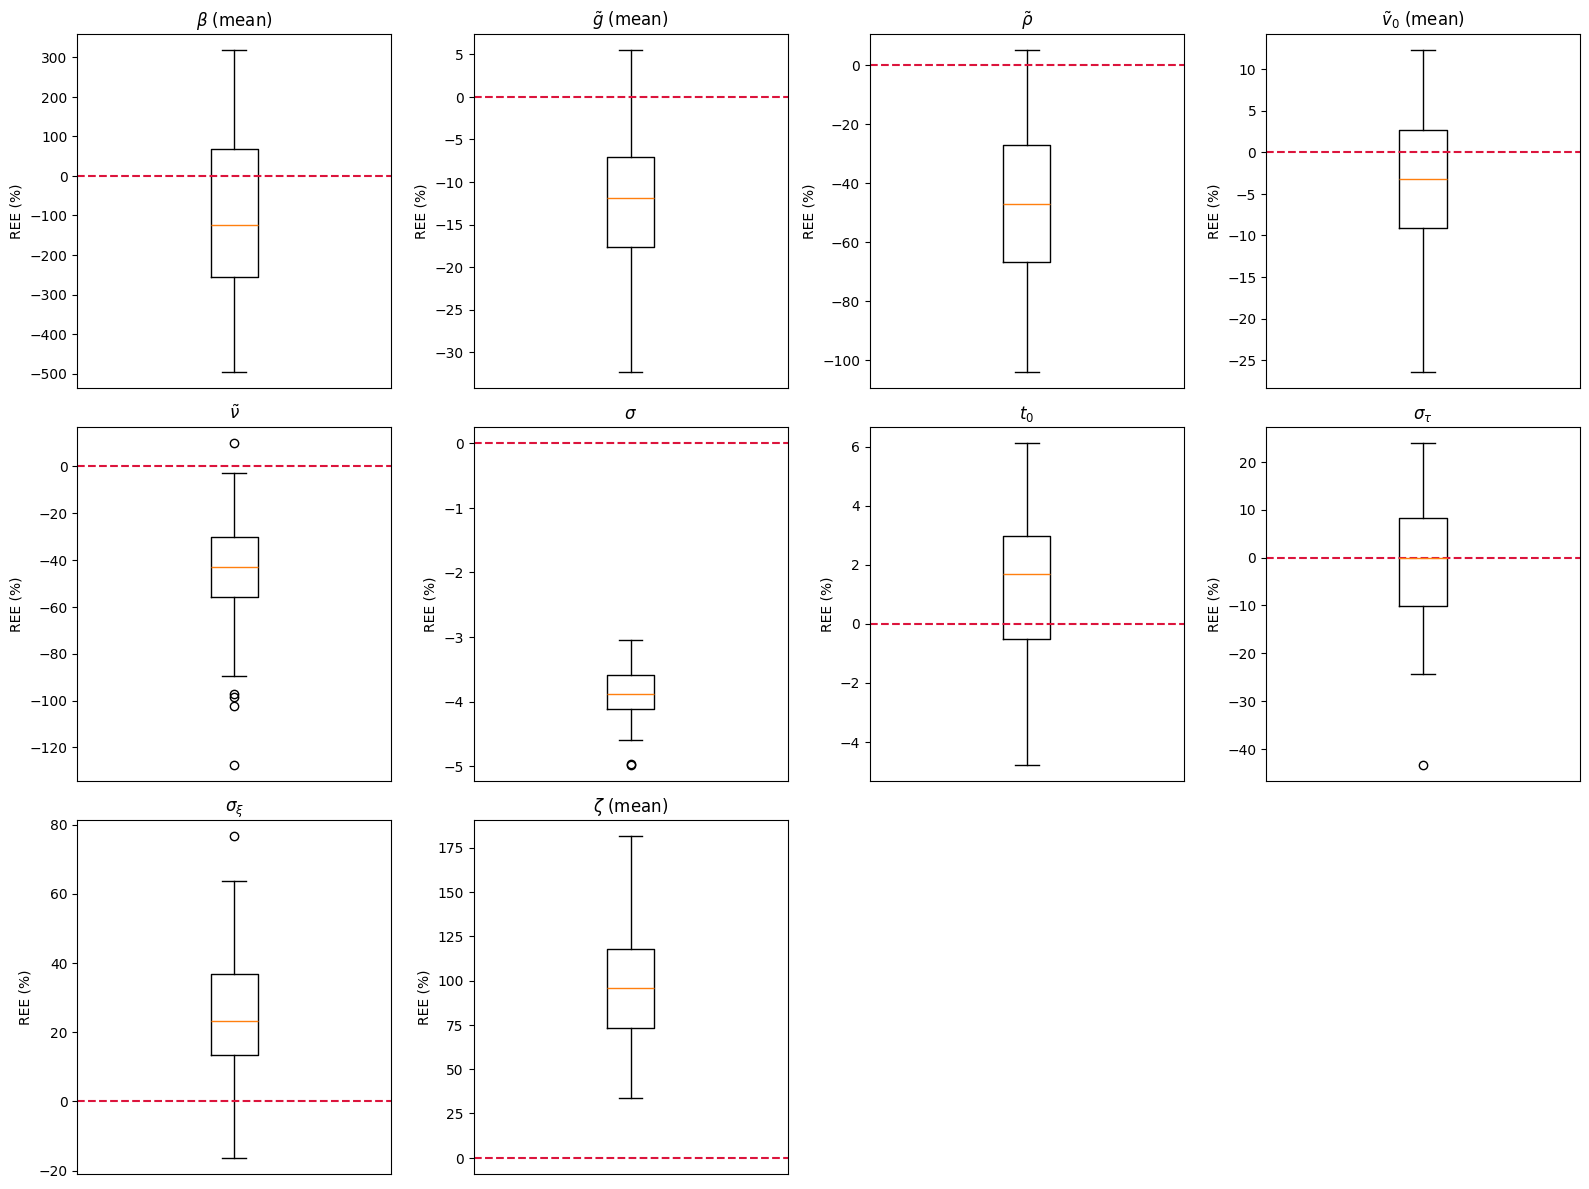
\includegraphics[width=0.7\textwidth]{figures/REE_all.png}
  \caption{Relative error of estimation (REE) for all parameters.}
  \label{fig:ree_all}
\end{figure}

\subsubsection{Individual random effect recovery}

The recovery of individual random effects $(\xi_i, \tau_i)$ is assessed through the ICC(3,1) and Bland-Altman analyses pooled across the $M$ repetitions. Scatter plots of personalised against true values are shown in Figure~\ref{fig:param_comparison}, and the corresponding Bland-Altman plots in Figure~\ref{fig:bland-altman}.

For the log-acceleration factor $\xi_i$, the mean ICC(3,1) across repetitions is $0.841 \pm 0.013$ and the corresponding Pearson correlation is $0.877 \pm 0.012$. For the time-shift $\tau_i$, the ICC(3,1) is $0.856 \pm 0.019$ and the Pearson correlation is $0.874 \pm 0.014$. Both statistics are reported because, as discussed in Section~\ref{sec:metrics}, the Pearson correlation is insensitive to affine shifts of the estimates and may overstate the quality of agreement when a systematic rescaling is present. Here, the ICC values of approximately $0.85$ for both parameters confirm that the personalisation procedure consistently identifies the relative ordering of patients along the disease timeline.

The scatter plots in Figure~\ref{fig:param_comparison} reveal some distortions. For $\xi_i$ (left panel), the linear regression line has a slope greater than one. Extreme values of the log-acceleration factor are systematically amplified in the personalised estimates, producing an expansion of the estimated distribution relative to the true one. This expansion is the individual-level counterpart of the population-level overestimation of $\sigma_\xi$: the fitted model assigns a larger variance to the prior on $\xi_i$ and thus, the posterior for each individual is wider and its mean is pulled further from zero, inflating the apparent spread. For $\tau_i$ (right panel), the regression slope is less than one, producing a contraction of the estimated time-shifts toward the population mean $t_0$. This is a standard Bayesian shrinkage effect, whereby the prior $\tau_i \sim \mathcal{N}(t_0, \sigma_\tau^2)$ regularises individual estimates toward the population center. This effect is even more pronounced for patients with few observations or short follow-up whose individual data are less informative about their absolute position on the disease timeline.

\begin{figure}[htbp]
  \centering
  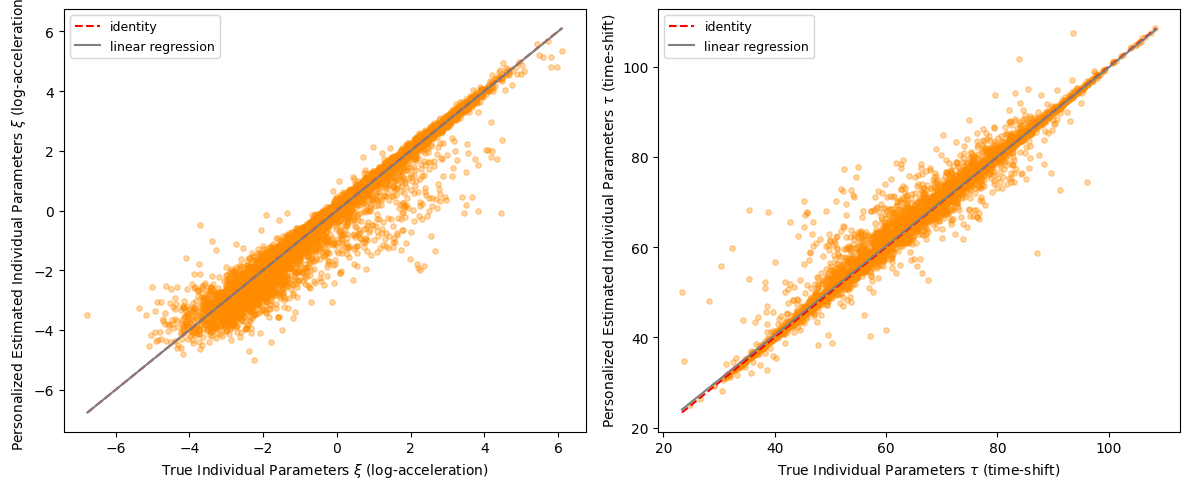
\includegraphics[width=\textwidth]{figures/parameters_comparison.png}
  \caption{Scatter plots of estimated vs. true individual parameters across all repetitions. The dashed line indicates the identity line of perfect agreement.}
  \label{fig:param_comparison}
\end{figure}

The Bland-Altman analysis in Figure~\ref{fig:bland-altman} completes this picture by examining the distribution of individual errors. For $\xi_i$ (left panel), the bias is negligible at $+0.009$, confirming that the personalisation step introduces no systematic offset in the estimated log-acceleration on average. No systematic trend is visible around the mean line, indicating the absence of proportional bias, the personalisation errors for $\xi_i$ do not grow with the magnitude of the true value.

For $\tau_i$ (right panel), the bias is $-0.080$ years, which is practically negligible relative to the inter-individual standard deviation $\sigma_\tau^* = 10.4$ years. The absence of a clear funnel-shaped or monotone pattern around the zero line indicates that the magnitude of the personalisation error does not grow systematically with the magnitude of $\tau_i$, so there is no evidence of proportional bias. 

Taken together, these results establish that the joint simulation and estimation pipeline is self-consistent: population parameters governing the longitudinal sub-model are recovered with good accuracy, individual parameters are personalised with meaningful concordance, and systematic biases remain confined to the survival-related and coupling parameters where finite-sample identifiability is inherently more challenging.

\begin{figure}[htbp]
  \centering
  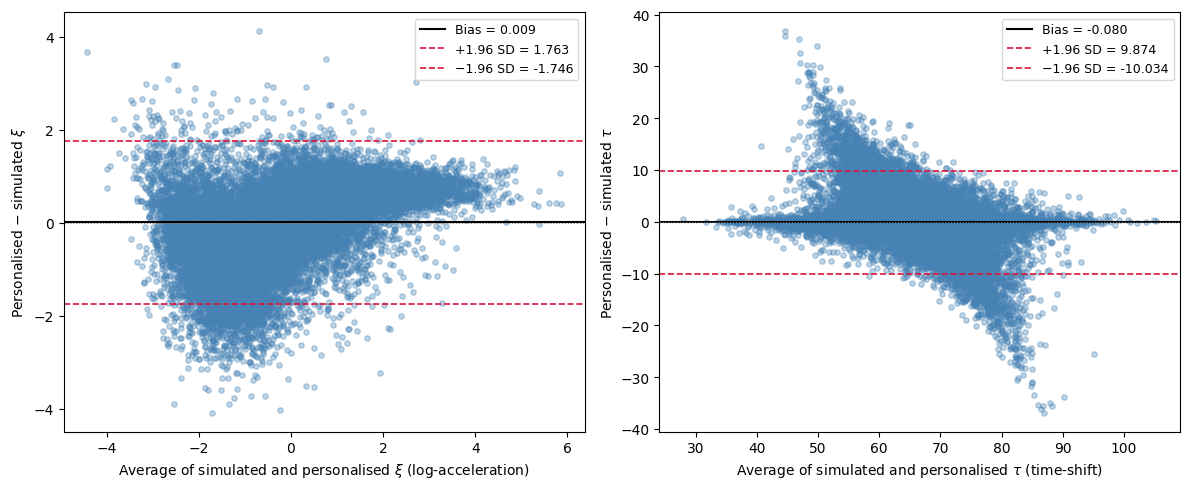
\includegraphics[width=\textwidth]{figures/bland-altman.png}
  \caption{Bland-Altman plots for $\xi$ (left) and $\tau$ (right). The solid line indicates the bias, and the dashed lines indicate the limits of agreement.}
  \label{fig:bland-altman}
\end{figure}


\newpage

\section{CS ONLY: Ethical and Sustainability Considerations} 

\subsection{Simulation as an Ethical Response to Patient Data Privacy}

A recurring concern throughout the internship was the handling of patient data from neurodegenerative disease cohorts. The datasets used to calibrate the reference models, such as PRO-ACT for amyotrophic lateral sclerosis or PULSE, contain sensitive longitudinal health information collected from individuals suffering from severe and often fatal conditions. Access to these datasets is governed by strict ethical protocols, data use agreements, and institutional review board approvals, and rightly so: the patients who consented to share their clinical trajectories did so in the expectation that their data would be used responsibly and that their privacy would be protected.

This constraint has direct consequences for research practice. Sharing fitted model parameters or reproducing a published result often requires access to the original dataset, which may not be redistributable. Collaborative method development across institutions is slowed by the administrative and legal overhead of data transfer agreements. Reviewers of a submitted paper cannot, in general, verify the reported results on the same data. These are not merely logistical inconveniences: they represent a structural tension between the scientific norm of reproducibility and the ethical imperative of data protection.

The simulation tools developed during this internship offer a partial but concrete resolution to this tension. A synthetic cohort generated under a calibrated model preserves the statistical properties of the original population, including trajectory shapes, individual variability, censoring patterns, and event rates, while containing no identifiable patient information whatsoever. No simulated individual corresponds to any real patient; the entire dataset is a probabilistic artefact of the fitted model. Such synthetic datasets can therefore be freely distributed alongside published code, included in software documentation, used in teaching workshops, and shared across institutions without any risk of re-identification or breach of consent.

During the internship, I came to appreciate that this property is not a secondary convenience but a genuine ethical contribution. The workshop I prepared and led on longitudinal data analysis with Leaspy relied entirely on simulated datasets, allowing participants to engage with realistic disease progression scenarios without any exposure to real patient data. More broadly, the availability of high-quality synthetic data lowers the barrier to entry for researchers who wish to develop or benchmark new methods but do not have direct access to clinical cohorts, thereby contributing to a more equitable and open research ecosystem.

This perspective also made me more attentive to the responsibilities that accompany the generation of synthetic data. A simulated dataset that faithfully reproduces the statistical structure of a real cohort could, in principle, be mistaken for real data or used to make clinical claims without the safeguards that govern actual patient studies. Ensuring that synthetic datasets are clearly labelled, that their provenance is documented, and that their limitations are explicitly stated is therefore an ethical obligation that accompanies the technical capability of simulation. In the Leaspy codebase, this concern was addressed through documentation and metadata conventions that distinguish simulated outputs from real observations.

\subsection{Computational Cost and Environmental Responsibility}

The validation study reported in this work required fitting $M = 50$ separate joint models from scratch, each involving $30\,000$ MCMC-SAEM iterations on a cohort of $N = 500$ synthetic patients, followed by a personalisation step of $5\,000$ iterations per patient. The total computational budget amounted to several days of continuous execution on institutional computing infrastructure. During the development phase, numerous additional runs were performed for debugging, hyperparameter exploration, and convergence diagnostics, multiplying the effective resource consumption well beyond the final reported experiment.

This experience confronted me with the environmental cost of simulation-intensive research. Each model fit consumes electrical energy, generates heat, and contributes to the carbon footprint of the research activity. While the individual energy consumption of a single MCMC-SAEM run is modest compared to, for instance, large-scale deep learning training, the cumulative effect of hundreds of exploratory and validation runs over a six-month internship is not negligible.

Several practical measures were adopted to mitigate this cost. First, the dense observation schedule used in the simulation study was deliberately chosen not only for statistical reasons but also because it reduces the number of SAEM iterations required for convergence, thereby shortening each run. Second, preliminary experiments on smaller cohorts ($N = 100$ or $N = 200$) were systematically conducted before committing to the full-scale study, in order to detect implementation errors or convergence failures early and avoid wasting computational resources on flawed configurations. Third, intermediate results and fitted model objects were systematically saved to disk, so that a failed or interrupted run could be resumed or analysed without repeating the entire computation. These practices, while individually modest, collectively reduced the total number of unnecessary computations by a meaningful factor.

\subsection{Open-Source Software for Clinical Research: Reliability and Responsibility}

Leaspy is an open-source library intended to be used not only by its developers but also by applied researchers, clinicians, and students who may not have the statistical or computational expertise to audit the implementation in detail. During the internship, I contributed to several aspects of the software beyond the core simulation pipeline: reviewing pull requests, writing and improving unit and functional tests, and strengthening the documentation. These activities, which occupied a substantial fraction of the internship time, brought me into direct contact with the question of software responsibility in a clinical research context.

The stakes are significant. A bug in the simulation algorithm could produce synthetic datasets whose statistical properties do not match the intended model, leading to incorrect conclusions in a validation study. An error in the \texttt{estimate} method could bias the survival predictions used for patient stratification. A poorly documented function could be misused by a researcher unfamiliar with the model assumptions, producing results that are technically valid but scientifically misleading. In all these cases, the consequences extend beyond the software itself: they affect the scientific conclusions drawn from the software and, ultimately, the clinical decisions informed by those conclusions.

This awareness shaped my approach to software development throughout the internship. Every new feature was accompanied by unit tests designed to catch regressions, and functional tests that verified end-to-end consistency against known reference values. Code reviews were conducted not only for correctness but also for clarity, because a piece of code that is correct but opaque is a latent source of future errors when modified by another contributor. Documentation was written with the assumption that the reader might be a biostatistician or a neurologist rather than a software engineer, and therefore needed to explain not only what a function does but why it does it and under what assumptions.

This dimension of the internship was formative in a way that I had not anticipated. My academic training in statistics and machine learning had emphasized the importance of methodological rigour, but had given comparatively little attention to the software practices that translate methodological ideas into reliable, usable tools. Working on Leaspy taught me that the gap between a correct mathematical formulation and a correct software implementation is wide, and that bridging it requires a distinct set of skills: systematic testing, defensive programming, clear documentation, and a culture of peer review. These are not peripheral concerns but core competencies for any researcher whose work involves computational methods, and I expect them to remain central to my professional practice in the years ahead.

\newpage

\section{TBD: Preliminary Work on the Phd Subject}
TODO
\newpage

\section{Conclusion}

This internship addressed a central methodological and software challenge for the Leaspy library: providing simulation and evaluation tools for complex non-linear mixed-effects models, and more specifically for the joint model linking longitudinal and survival data. In a context where real clinical datasets never provide access to the true latent disease stage or to the true individual random effects, simulation constitutes an indispensable instrument both for validating statistical procedures and for testing software implementations under controlled conditions.

The main contribution of this work was the development and integration of a simulation pipeline for the joint model within the Leaspy codebase. This required extending the existing logic of the library to support the generation of event times alongside longitudinal trajectories, handling censoring constraints, adapting the \texttt{estimate} method to return survival-related quantities, and generalizing the framework to competing events. These developments made it possible to simulate synthetic cohorts in a way that is coherent with the mathematical structure of the joint model and with the design principles of the Leaspy API.

A second important contribution was the implementation of a simulation-based validation strategy aimed at evaluating the self-consistency of the full pipeline. By repeatedly simulating datasets from a reference fitted model and re-estimating the parameters, the study assessed the recovery of both population parameters and personalized individual random effects. The results show that the main longitudinal parameters and the subject-level time-shift and acceleration effects are recovered with good accuracy in the considered setting. At the same time, some parameters related to survival and latent-source couplings exhibit substantially larger estimation errors, highlighting the practical difficulties of identifying second-order effects in moderately sized cohorts. These findings are informative not only for the specific implementation developed during the internship, but also more generally for the statistical use of the joint model.

Beyond the work described in detail in this report, the internship also involved a broader contribution to the life of the project: reviewing pull requests, strengthening the test suite with unit and functional tests, improving parts of the documentation, and preparing and leading a workshop on longitudinal data, with a particular focus on simulation. These activities were essential to ensure that the developed features are not only methodologically relevant, but also maintainable, documented and usable by other contributors and end users.

Overall, this internship provided an opportunity to work at the interface between statistics, machine learning and scientific software engineering, in a highly interdisciplinary research environment. It also illustrated a key aspect of modern methodological research: proposing a model is not sufficient; one must also provide the computational tools, validation procedures and software standards that make its use reliable and reproducible. In that respect, the work carried out during these six months contributes to making Leaspy a more robust and more complete platform for longitudinal disease progression modeling.

Several perspectives naturally follow from this work. On the methodological side, future simulation studies could investigate more systematically the effect of sample size, censoring intensity, visit sparsity, or model misspecification on parameter recovery. On the software side, the simulation framework could be extended further, for instance by allowing more flexible visit-generation schemes, richer noise models, or closer alignment between continuous-time event generation and the current grid-based implementation. More broadly, the tools developed here may support future benchmarking studies, educational uses, and the generation of privacy-preserving synthetic datasets for open research. These perspectives make simulation not only a technical feature of Leaspy, but also a strategic component of its future development.
\newpage

% Bibliography 
\bibliographystyle{plain}
\bibliography{bibliography}

\end{document}
